Modern analytics environments grapple with the complexity of managing diverse datasets originating from various applications or collected by autonomous agents. Over the last decade, Business Analytics (BA) has evolved significantly through four eras: Analytics 1.0 to Analytics 4.0. In Analytics 1.0, traditional analytical tools were used for decision-making until 2005. The emergence of Big Data marked Analytics 2.0, led by companies like Google and Facebook. Analytics 3.0 combined Big Data and small data analytics for decision support and product creation, while Analytics 4.0, the current era, emphasizes autonomy and democratizing analytics tasks with new job roles like citizen data scientists and business translators alongside quantitative analysts and data scientists \cite{Aleksic2019}. The definition of big data has evolved rapidly, causing confusion among executives due to varying perspectives on its characteristics. The Three V's - Volume, Variety, and Velocity - serve as a common framework to describe big data, representing its high-volume, high-velocity, and high-variety nature. Other dimensions like Veracity, Variability, and Value have also been considered in defining big data. Universal benchmarks do not exist, and the definition depends on factors such as the firm's size, sector, and location. The Three-V tipping point signifies when traditional data management and analysis technologies become inadequate for handling big data efficiently \cite{GANDOMI2015137}. The high-variety datasets exhibit heterogeneity not only in their semantics but also in the data structures that store them and the systems that manage and process them. Utilizing Big Data poses significant challenges for managers across different business functions. To leverage its potential, a new profession, data scientist, with specific skill sets is necessary. This heterogeneity has created the need for different roles in the analytics environment including developers, data engineers, data scientists, data analysts, business users, and data regulation officers, that undertake different analysis projects, ranging from traditional business intelligence to data exploration, data mining, and prediction \cite{Mauro2016}. As of 2016, there was a shortage of approximately 190,000 data scientists in the United States alone \cite{Aleksic2019}.

To effectively address the challenges posed by this diverse landscape, multiple data systems and analysis platforms must coexist, integrated, and federated. While data warehousing has been a common approach, it becomes rigid in rapidly changing data environments. Furthermore, there is a need for techniques that allow the creation of late-bound schemas on data that may be persisted but rarely processed or even never processed. This requirement becomes particularly prevalent in dynamic data infrastructures where analysis objectives change with agility. In such environments, creating comprehensive classical integrated schemas encompassing structured, semi-structured, and unstructured data proves to be not only highly time and resource-intensive but often unattainable within the time constraints of analysis \cite{abadi2016beckman}. As an alternative, many production environments adopt a programming language (e.g., Python, R, Scala) to ad-hoc extract, transform, and assemble data, such as in dataframes, to swiftly build models or reports. Python is a popular open-source programming language supported on various platforms. It offers thousands of third-party packages, including NumPy, Scikit, and Pandas, which are essential for machine learning and data mining tasks. These packages provide support for scientific computing, data preprocessing, modeling, and analysis, making Python user-friendly and suitable for quick problem analysis \cite{Bhadani2016}. Although dataframe libraries in R and Python have achieved considerable success, they encounter performance problems when dealing with moderately large datasets. Additionally, there is considerable uncertainty about the precise meaning or interpretation of dataframe semantics \cite{petersohn2020scalable}. Moreover, this approach lacks data exploration capabilities for end-users, as generating new datasets necessitates creating entirely new programs. 

Python and R offer support for dataframe abstraction, which is a functional interface better suited for developers and data scientists implemented through data science notebooks. Dataframes are more tolerant of unknown data structures and are widely used in data exploration. They possess several characteristics that make them attractive for this purpose: intuitive data model, query language versatility, dataframes offer a query language that bridges various data analysis modes, including relational operations (e.g., filter, join), linear algebra (e.g., transpose), and spreadsheet-like functions (e.g., pivot), incrementally composable query syntax and native embedding in host languages \cite{perez2015project}. Pandas, the library within Python, has been a popular choice for data exploration. However, the rich API of pandas has led to redundancies, making it challenging for users to manually plan queries and optimize performance. The complexity of the API also hinders traditional query optimization techniques. Additionally, pandas' performance breaks down when processing moderate volumes of data that exceed memory limits \cite{petersohn2020scalable}.

As a response to that issue, we propose the following research question.
\textbf{Research question:} \textit{Can a virtual data machine that works on top of the organization data infrastructure as a layer that establishes on-demand connections with the required data sources offer easy dataframe queries formulation by no programming expert users and competitive performance to other traditional python-notebook-based solutions?}

To tackle this challenge, we propose the Data Virtual Machine (DVM), a novel graph-based conceptual model based on entities and attributes, concepts that users intuitively understand. The fundamental idea behind the DVM is both simple and powerful: given a computation C with an output (o1, o2), where o1 belongs to attribute domain A and o2 belongs to attribute domain B, the output of C can be represented as a mapping between A and B. This mapping can be depicted in a graph with nodes A and B and edges representing the mappings as manifested by C's output, which can encompass queries, scripts, programs, and more. The DVM introduces agile and on-demand modeling capabilities, allowing end-users to easily define computations over the data sources, covering relational and non-relational data, streams, and stand-alone programs, visually. As a result, the DVM is automatically generated, reflecting a collection of computations based on their output. This approach diverges from traditional data integration techniques, where the focus is on settling on a fixed schema and then defining data processing tasks to populate or refresh it in data warehousing, or utilizing wrappers to bind data with a virtual schema in case of mediators/virtual databases. Instead, the DVM fits existing data to dynamically constructed schemas, providing greater flexibility and adaptability to evolving analysis requirements. Additionally, it facilitates easy and intuitive querying, enabling non-database experts, such as data scientists and statisticians, to express queries using a high-level query definition language similar to SQL. The DVM's visualization-driven approach effectively hides query optimization and structural details, enhancing usability.

This paper's contributions encompass the introduction of the DVM as a novel conceptual model, a declarative approach to dataframing in analytics environments, and the proposal of an algebraic framework for efficient query evaluation along with concurrency and parallelization optimizations in the calculations. A case study validates the effectiveness of DVMs and the visual DVM query language in effortlessly creating advanced dataframes analysis that would otherwise require programming skills. Moreover, a benchmarking of the DataMigler tool is performed against the traditional Python-notebook-based implementations that demonstrate the superior performance of DataMigler in the query evaluation.

The subsequent sections elaborate on key analytics environment concepts, present the DVM's formal definition and intuitive explanation, introduce DVM dataframe queries and the algebraic framework for their evaluation, discuss query evaluation and optimization, showcase a case study as a proof-of-concept, benchmarking of the tool, and conclude with limitations and future directions for this innovative approach.

\subsection{Motivation example setup queries}

To execute our experiments and showcase the usage of a DVM we used the data from the model shown in Figure \ref{dvm2}. They represent taxi rides in New York City in 2022, connected to relevant weather and traffic data. The weather attributes shown in the model, \texttt{snowProb, humidity, rainProb, temperature, datetime, location},  were collected by the \href{https://www.visualcrossing.com/}{Visual Crossing} service for the year 2022 in the city of New York. The traffic data, \texttt{meanSpeed, meanCongestion, datetime, location}, were gathered from \href{https://opendata.cityofnewyork.us/}{NYC Open Data}, which publishes free, public, up-to-date datasets from the city of New York. The attributes concerning the taxi rides, \texttt{DOLocation, PULocation, passengerFare, driverTip, requestDatetime, triverPay, tripTime, tripMiles, airportFee}, were taken from a dataset published by the \href{https://www.nyc.gov/site/tlc/about/tlc-trip-record-data.page}{NYC Gov} website. The datasets from NYC Open Data and NYC Gov used an area code to describe location. In order to match datetime and location data with the other data sources, the area codes were mapped using a complementary dataset to NYC districts and specific areas. After the mapping, the \texttt{requestDatetime} and \texttt{PULocation} from the taxi data attributes were concatenated and hashed using the MD5 hashing method to produce the \texttt{locationDatetimeID} attribute The same was done to the \texttt{location} and \texttt{datetime} attributes for weather and traffic. This action produced a primary attribute that connected all different data sources. Finally, the \texttt{passengerReview} attribute and the \texttt{driverID, gender, vehicleModel, driverUID} were added from two \href{https://www.kaggle.com/}{Kaggle} dataseta that contained customer reviews and driver data for Uber rides. Because most of our data was in CSV form we did some refactoring to test our assumptions under different kinds of data sources. Firstly, the dataset containing the taxi rides was turned into a PostreSQL relational database. The database contained four tables \texttt{trip\_details, trip\_time, trip\_speed} and \texttt{trip\_location}. The attributes were split between those tables and had as primary key a unique integer number called \texttt{intID} and as secondary key the \texttt{locationDatetimeID}. A schema representation can be seen in Figure \ref{schema}. For the rest of the data, the passenger review data were turned in XML format, the weather data in Excel and the traffic and Uber drivers data were kept in a CSV format.

\begin{center}
    \begin{figure}[h]
        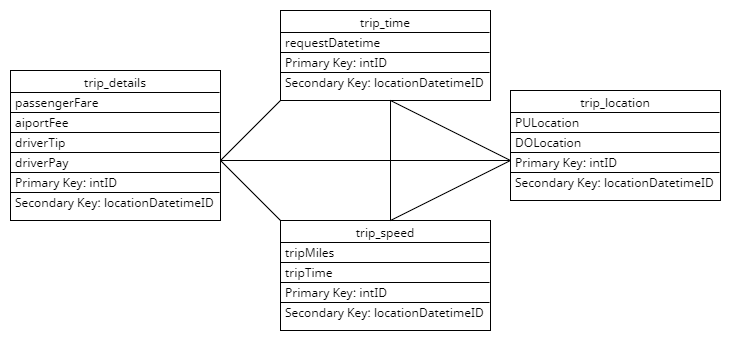
\includegraphics[scale=0.3]{figures/schema.png}
        \caption{Schema representation of taxi rides relations database.}
        \label{schema}
    \end{figure}
\end{center}

It is worth noting that the datasets contained many more attributes than the ones shown in Figure \ref{dvm2}. The purpose of the graphical representation is to highlight the main fields used in our analysis and create a comprehensive conceptual image. Also, the names of the attributes shown in Figure \ref{dvm2} do not match accurately to the ones in the datasets. This was done in order to have more easily understandable naming conventions across the different data sources in the conceptual image that we created.

\begin{center}
    \begin{figure}[h]
        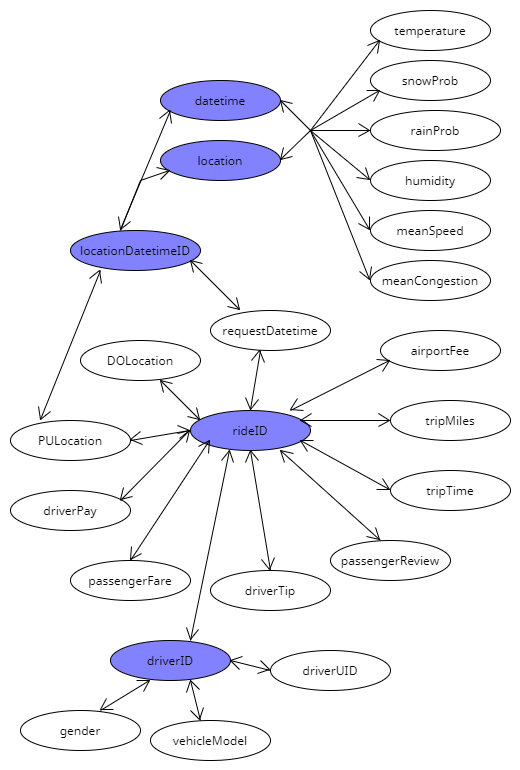
\includegraphics[scale=0.3]{generalDVMView}
        \caption{DVM view of our data.}
        \label{dvm2}
    \end{figure}
\end{center}

With that in mind, a dataframe query over the data is defined by Chatziantoniou et. al. (2022)\cite{chatziantoniou} in Definition 3.2.

\textit{Definition 3.2:} \textbf{[Dataframe Queries]} Given a DVM \(G = \{A, S\}\), a dataframe query is a tree structure \(Q\), defined as:

\begin{itemize}
    \item each node \(N\) of \(Q\) has a \textit{name} and a \textit{label}: the name is unique within \(Q\) and the label is an attribute of \(G\); these are denoted as \(N.name\) and \(N.label\) respectively
    \item for each edge \(N \to N^'\) in \(Q\), there exists an edge: \(label(N) \to label(N^')\) in \(D\)
    \item each edge \(e\) of \(Q\) is annotated with a list of transformations, called the \textit{transformations string}, denoted as \(e.transformations\)
    \item each node \(N\) of \(Q\) is annotated with the \textit{selection condition}, which is either the special value \texttt{'True'} of a python like logical expression, where \(N\) and any of \(N\)'s children may appear as identifiers within this expression; the selection condition of \(N\) is denoted as \(N.selection\)
    \item each node, except the root, has an \textit{output label}, which has the value \texttt{'true'} or \texttt{'false'}; if the output label of a node is \texttt{'true'}, then all nodes in the path from the root to that node, except the root, must have a \texttt{'true'} output label; the output label of the node is denoted as \(N.output\)
\end{itemize}

An example of a dataframe query over the data described above can be seen in Figure \ref{query1}. The root could also be any other attribute of our data, such as \texttt{meanSpeed, passengerReview} etc. 

\begin{center}
    \begin{figure}[h]
        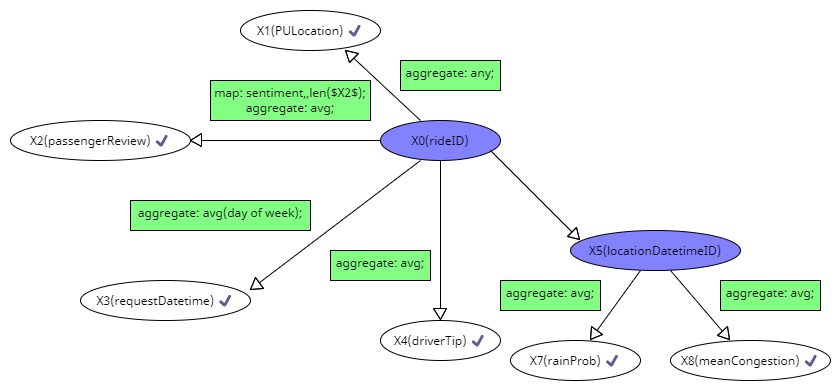
\includegraphics[scale=0.3]{query1}
        \caption{Query tree representation.}
        \label{query1}
    \end{figure}
\end{center}

The data that an organisation produces can be represented by a Data Virtual Machine (DVM), a conceptual model based on graphs. It provides for quick, ad hoc, on-demand data model development and offers schema flexibility. DVMs provide data sharing, data portability, and a single view of any entity. Data virtualization is an industry concept that is only starting to take off. Data is portrayed in a DVM as nodes and edges in a graph, where the nodes stand in for attributes and entities. By assigning attributes from various data sources to entities or by performing computations, DVMs can be swiftly created. They provide a formalism that makes it possible for non-IT experts to participate in dataframing duties and they enable data exchange and data portability. DVMs can be created quickly and represent the aggregate of calculations carried out on the data infrastructure. The data retrieval operations or computations made on the already-existing data determine the schema of a DVM. They offer an algebraic framework for query evaluation with proven advantages and permit declarative and visual description of dataframes\cite{chatziantoniou}.

\subsection{Data Virtual Machines}

To understand how a DVM works, it can be thought of as an altered ER (Entity-Relationship) model. In an ER model, entities are represented at a higher level, and relationships are depicted between entities using relationship modeling constructs. However, in a DVM, all attributes are \textit{derived} and \textit{multi-valued}, and entities are represented by their \textit{primary attributes}. This means that in a DVM, each node can be considered either as an entity or an attribute, depending on the analysis perspective. A DVM consists of \textit{mappings}, that are represented as edges, between \textit{attribute domains}, that are represented by nodes. Mappings appear as data processes with a 2-dimensional output (the attribute domains)\cite{chatziantoniou}.

For example, in an ER model, attributes are directly associated with entities, and relationships are defined separately. In contrast, in a DVM, attributes are derived through computations and bound to entities via their primary attribute. The primary key of an ER entity now represents the entity itself as a node, associated with other nodes that represent the entity's attributes.

While ER models follow a top-down approach, starting from conceptual design and going towards a logical model, DVMs follow a bottom-up approach, starting from existing data and constructing a conceptual model based on the computations performed on that data\cite{chatziantoniou}.

\textit{Definition 3.1:} \textbf{[Data Virtual Machines]} Assume a collection \(A\) of \(n\) domains \(A_1, A_2, ..., A_n\) called \textit{attributes}. Assume a collection \(S\) of \(m\) multisets \(S_1, S_2, ..., S_m\), where each multiset \(S\) has the form: \(S = \{(u, v): u \in A_i, v \in A_j, i, j \in \{1, 2, ..., n\}\}\), called \textit{data processing tasks}. For each such \(S \in \{S_1, S_2, ..., S_m\}\) we define two key-list structures, \(K^S_i_j\) and \(K^S_j_i\) as:
\begin{itemize}
    \item[] \(K^S_i_j\): for each \(u\) in the set \(\{u: (u, v) \in S\}\) we define the list \(L_u = \{v: (u, v) \in S\}\) and \((u, L_u)\) is appended to \(K^S_i_j\). \(K^S_j_i\) is similarly defined.
\end{itemize}
The DVM is a multi-graph \(G = \{A, S\}\) constructed as:
\begin{itemize}
    \item each attribute becomes a node in \(G\)
    \item for each data processing task \(S\) we draw two edges \(A_i \to A_j\) and \(A_j \to A_i\), labeled with \(K^S_i_j\) and \(K^S_j_i\) respectively.
\end{itemize}
The key-list structure that corresponds to an edge \(e: A_i \to A_j\) is denoted as \(KL(e\), with schema \((A_i, A_j)\)\cite{chatziantoniou}.

\textit{Example 3.1:} Assume two attributes, \texttt{rideID} and \texttt{locationDatetimeID} and the output of te SQL query "\texttt{SELECT rideID, locationDatetimeID FROM taxiRides}" that maps taxi rides and datetime specific locations. The key-list structure of the nodes and edges created by the attributes can be seen in Figure \ref{dvm1}.

\begin{center}
    \begin{figure}[h]
        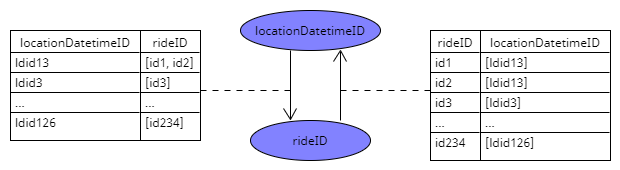
\includegraphics[scale=0.4]{erToDVMExample}
        \caption{ER to DVM representation.}
        \label{dvm1}
    \end{figure}
\end{center}
